\section{Background}\label{sec:background}
\localtableofcontents
\subsection{Imaging systems}\label{subsec:imaging-systems}
\begin{figure}[!htbp]
	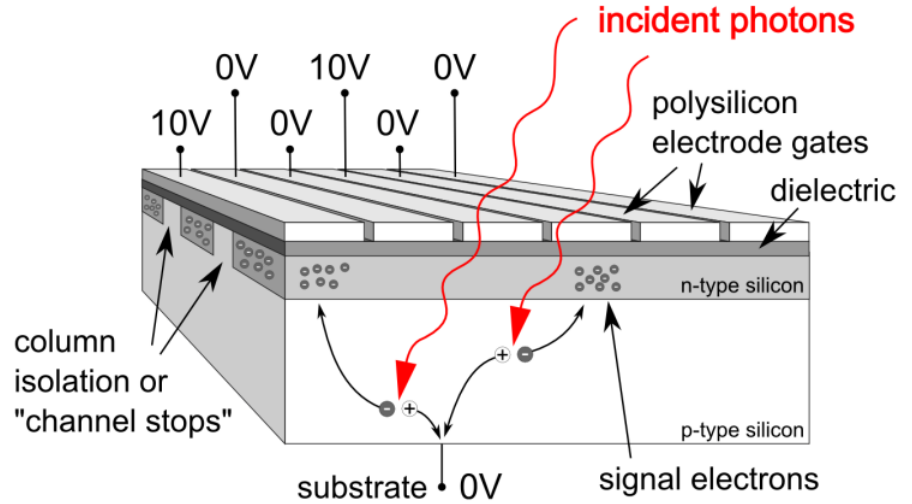
\includegraphics[width=\linewidth,keepaspectratio]{figures/background/bccd.png}
	\caption{CCD buried channel MOS capacitor \cite{finaltestguideline}.}
	\label{fig:mos-cap}
\end{figure}

We begin with a practical discussion of imaging systems.
%
An imaging system consists of an imaging sensor and optics. 
%
An imaging sensor is a device that converts an optical image into a digital signal.
%
Charge-coupled devices (CCD) and complementary metal-oxide-semiconductor (CMOS) devices are the most common imaging sensors; CCDs have better performance while CMOS devices are newer and less expensive.
%
A third type that's of particular interest to us is the microbolometer, which is used as a sensor in thermal cameras.

\subsubsection{CCD Devices}

CCDs consist of two components: an imaging component and a readout component.
%
The imaging component is arranged with every third stripe of electrode tied electrically to form three sets of equipotentials.
%
These equipotentials taken together constitute a \textit{vertical register} (VR) (see figure~\ref{fig:ccd-array}).
\begin{figure*}[!htbp]
	\centering
	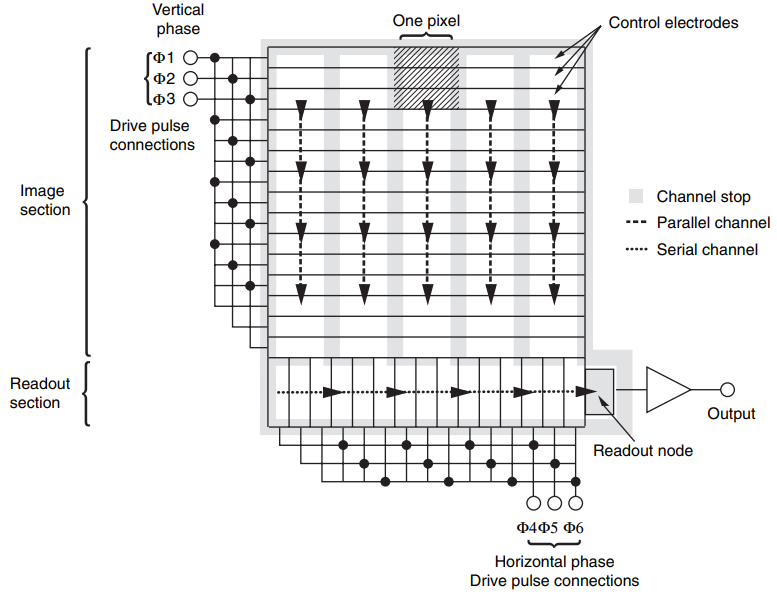
\includegraphics[width=.8\textwidth,keepaspectratio]{figures/background/ccd_array.png}
	\caption{CCD array with both image and readout components \cite{pawley1995handbook}. Note that all electrodes intersecting \(\Phi i\) for some \(i\) are at the same potential (voltage).}
	\label{fig:ccd-array}
\end{figure*}
%
A vertical register moves the collected photoelectrons down one electrode line at a time, using charge coupling, with the aid of channel stops (which function to prevent diffusion of charge across channels).

More precisely the imaging component of a CCD consists of densely packed two-dimensional arrays of buried channel\anote{buriedchannel} metal-oxide-semiconductor (MOS) capacitors (see figure~\ref{fig:mos-cap}).
%
Individual MOS capacitors are biased by a gate voltage such that a potential well develops in the n-type\anote{ntype} silicon.
%
This potential well acts as a storage system for charge induced by the inner photoelectric effect\anote{innerphotoelectric}.
%
When photons are incident on a MOS capacitor some of the photons are absorbed at the surface, some are scattered at the surface, and some are transmitted into the bulk material.
%
Those photons that are transmitted interact with electrons in the valence band of the silicon substrate and thereby excite them into the semiconductor's conduction band.
%
This creates electron-hole pairs that either diffuse or recombine (in the silicon).
%
For high-quality silicon, the lifetime of such a pair is several milliseconds (before recombination) \cite{scientificccd}.
%
The electrons of the electron-hole pairs (that do not recombine) then diffuse into the potential well, while the holes migrate to the grounded substrate (i.e., out of the sensor).
%
Electrons created in this way are called \textit{photoelectrons}.

Suppose the VR is in a state such that there's a collection of photoelectrons on each channel at equipotential \(\Phi1\) and only \(\Phi1\). Note this means \(\Phi2, \Phi3\) are at \(0\)v (again just as in figure~\ref{fig:mos-cap}). The VR mechanism that shifts collected charge operates as follows:
\begin{framed}
\begin{enumerate}
	\item \(\Phi2\) is positively biased to \(10\)V. This causes redistribution of charge such that it is diffused underneath both \(\Phi1\) and \(\Phi2\).
	\item \(\Phi1\) is set to \(0\)v. This concentrates the charge exclusively under \(\Phi2\).
	\item The same redistribution is repeated vis-à-vis \(\Phi2, \Phi3\) and \(\Phi3, \Phi1\).
	\item The entire process repeats thereby shifting the charge three electrode lines (or one pixel row) at a time.
	\item At the bottom of the image section \(\Phi3\) transfers all charge to the horizontal register which functions much like the VR except faster.
\end{enumerate}
\end{framed}
%
An obvious challenge faced by this system is how to prevent errant charge from accumulating out of sync with the shift process, i.e., how to prevent new photoelectrons from being produced at intermediate electrode lines while far lines are being shifted.
%
The solution is to have interstitial dedicated shift channels in between columns of sensors, with the shift channels being masked off from exposure to light.
%
This type of reading is called \textit{interline transfer} because the accumulated charge is first moved one line over, into the shift channels.
%
Naturally, interline transfer shrinks photosensitive area by half and despite possible solutions (e.g, micro-lenses being used to focus most of the light onto the unmasked sensors) this is one of the drawbacks of CCDs relative to CMOS devices.

\subsubsection{CMOS Devices}

CMOS devices consist of arrays of photodiodes (see figure~\ref{fig:photodiode.png}).
\begin{figure}
    \centering
    \begin{subfigure}[b]{0.49\textwidth}
        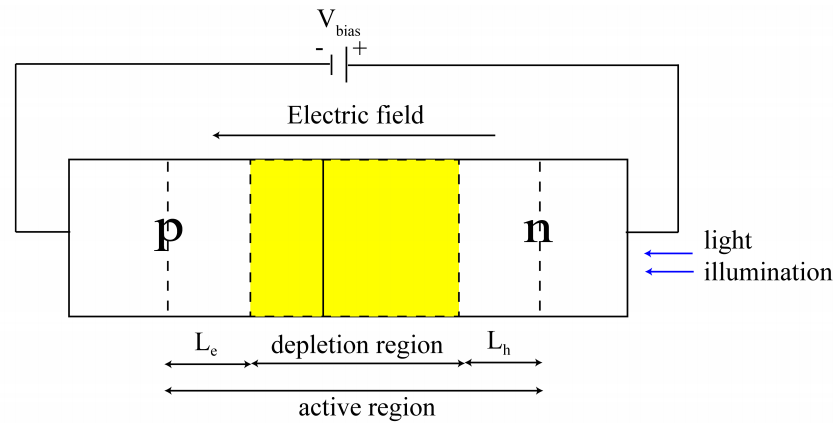
\includegraphics[width=\linewidth,keepaspectratio]{figures/background/cmos/photodiode.png}
        \caption{Photodiode schematic. L\textsubscript{e}, L\textsubscript{h} are electron, hole diffusion lengths respectively\cite{Xu2015FundamentalCO}.}
        \label{fig:photodiode.png}
    \end{subfigure}
    \vskip\baselineskip
    \begin{subfigure}[b]{0.49\textwidth}
        \center
        
\includegraphics[width=.8\linewidth,keepaspectratio]{figures/background/cmos/3t_pixel.png}
        \caption{Three transistor pixel. M\textsubscript{rst} is the reset transistor (enabling the photodiode to dump charge), M\textsubscript{sf} buffers the charge on the photodiode (so that it can be read without loss), and M\textsubscript{sel} enables a whole row of pixels to be read simultaneously (since all pixels in a physical row are tied to the same row line).}
        \label{fig:3tpixel}
    \end{subfigure}
    \caption{CMOS components.}
\end{figure}
A photodiode is a \textit{p-n junction}\anote{pnjunction} operated in reverse bias mode\anote{reversebias}.
%
When a photon of sufficient energy is absorbed by the diode, it creates an electron-hole pair (as a result of the photoelectron effect).
%
If the creation event happens within the active region then the hole migrates out through the p-type material and the electron migrates out through the n-type material.
%
This establishes a \textit{photocurrent} that can be interrogated by a reading circuit (see figure~\ref{fig:3tpixel}).

CMOS sensor arrays do not shift the charge from row to row like CCD arrays.
%
In a CMOS sensor array, each pixel contains a transistor M\textsubscript{sel} controlled by the voltage applied across a row (see figure~\ref{fig:cmosarray}).
%
In order to read one row of pixels, a rowline is raised high to turn on (close) all the M\textsubscript{sel} transistors in the row.
%
This brings the signals from all the pixels in that row to the shift register below by way of the column lines.
%
The shift register then outputs the values of the pixels.

The high number of transistors needed per pixel in CMOS arrays has only recently become feasible for semiconductor foundries to manufacture.
%
This, along with such artifacts as the rolling shutter effect produced by rowline reading, are some of the drawbacks of CMOS devices relative to CCD devices.
%
Despite this CMOS devices have become the most common imaging system in consumer goods such as cell phones and digital cameras due to their relatively simple mechanics.
\begin{figure}[!htbp]
	\center
	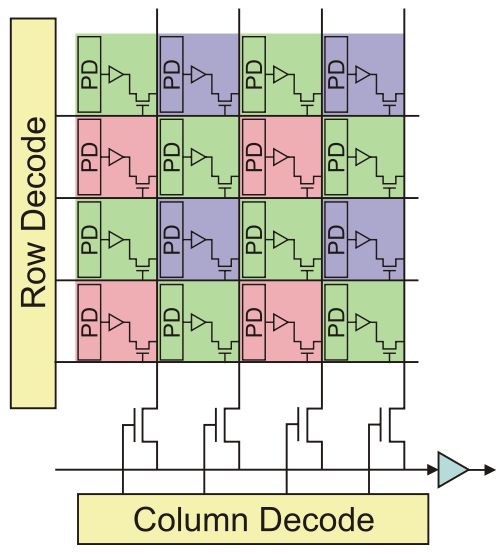
\includegraphics[width=.8\linewidth,keepaspectratio]{figures/background/cmos.png}
	\caption{CMOS array of red, green, and blue pixels.}
	\label{fig:cmosarray}
\end{figure}

\subsubsection{Microbolometers}

Despite their ubiquity in visible spectrum devices, neither CCD arrays nor CMOS arrays can be adapted to capture any portion of the infrared spectrum.
%
A microbolometer, on the other hand, measures the power in the infrared by exposing a thermistor\anote{thermistor} to the incident light.
%
\begin{figure}[!htbp]
	\center
	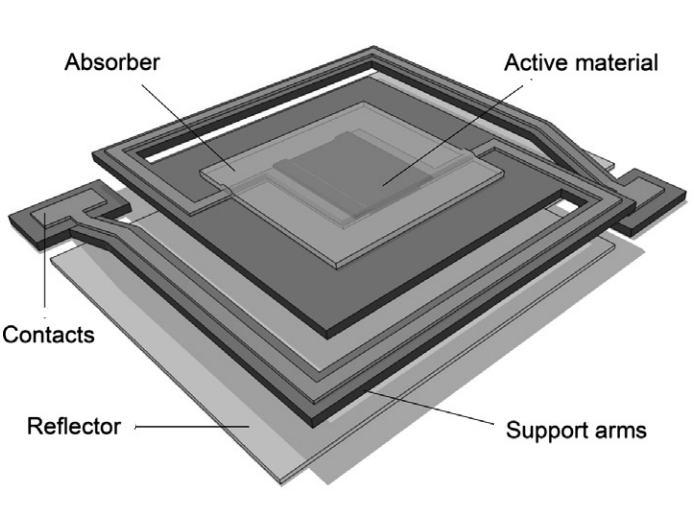
\includegraphics[width=\linewidth,keepaspectratio]{figures/background/microbolometer2.png}
	\caption{Bridge structure of Honeywell microbolometer \cite{KESIM2014245}.}
	\label{fig:microbolometer}
\end{figure}
%
Since a thermistor's resistance changes as a function of its temperature, a key issue in the design of a microbolometer is the thermal isolation of the thermistor.
%
With the maturation of micro-machining techniques (such as for MEMS\anote{mems} devices) over the last few years efficient microbolometers have become possible.
%
There are now many consumer thermal cameras on the consumer market powered by two-level microbolometer pixels consisting of a thermo-sensitive component suspended above (and insulated from) silicon (see figure~\ref{fig:microbolometer}).

These pixel packages are evacuated in order that they have good conduction, convection, and radiation heat transfer properties.
%
The actual thermo-sensitive component consists of a thermistor, an absorber (which aids in the transfer of heat to the thermistor), and a reflector that creates a Fabry–Pérot optical cavity\anote{fabryperot} (typically \({\sim}\lambda/4\) \cite{bolometer}) that traps the infrared light.
%
Typical materials for the thermistor are vanadium oxide and amorphous silicon owing to their high temperature coefficients of resistance \cite{bolometer}, which, in effect transform small changes in temperature into large changes in resistance.
%
Measurements of the thermistor are performed by a read-out integrated circuit adjacent to the bridge in the silicon substrate.
%
It is plain to see that microbolometers are designed much differently from either CCD or CMOS arrays.
%
As a result of this fact, high-resolution infrared imaging systems are not as of yet available on the consumer market and hence our interest in applying super-resolution to images collected by such systems.
%
With that in mind, we now proceed to formalizing the problem of super-resolution.

\subsection{Interlude: Mathematical Notation}\label{subsec:notation}

Upper case plain latin \(X, Y\) each denote channel \(\times\) row \(\times\) column \textit{tensors}\anote{tensor} representing LR and HR images respectively, with \((0, 0, 0)\) corresponding to the top left corner of the first channel of image.
%
Often for the sake of simplicity we consider grayscale images, in which case we omit the channel dimension.
%
\(D, H, F, G\) variously refer to functions that operate on images.
%
Bolded uppercase latin are reserved for batches of objects.
%
For example \(\bm{X}, \bm{Y}\) are batches of images, i.e., batch size \(\times\) channel \(\times\) row \(\times\) column tensors with \((0, 0, 0, 0)\) corresponding to the top left corner of the first channel of first image in the batch.
%
Bolded lower case latin such as \(\bm{x}, \bm{y}, \bm{z}\) denotes a conventional column or row vector.
%
Subscripts are used most often to indicate sequences (e.g., \(X_1, X_2, \dots\)) but occasionally indicate position (e.g., \((U_x, U_y)\)).
%
The \(L_2\) norm is indicated by unadorned \(\abs{\cdot}\).
%
All other norms are indicated by a subscript (e.g. \(\abs{\cdot}_1\) is the \(L_1\) norm).
%
New mathematical quantities are defined on first use by colon-equals \(\coloneqq\).
%
Hats denote computed estimators (e.g., \(\hat{X}\) is an estimate of \(X\) given noisy samples \(X_i\)).
%
All other notation is defined in situ.

\subsection{Imaging model}\label{subsec:imaging-model}

Figure~\ref{fig:bertrand} shows a conceptual model of the imaging process as carried out by an imaging system.
%
The input to the system is a natural scene that is in effect sampled by the imaging system.
%
In the idealized case, the sampling is done at (or above) the Nyquist rate and no aliasing occurs.
%
In practice there is noise and loss introduced at every step of the process: atmospheric turbulence plays a role at large distances, motion produces multiple views of the same scene but also induces blur, imperfections of the lenses further blur the image, and finally down-sampling by the sensor elements into pixels produces aliasing artifacts\anote{ccd}.
%
The noisy, blurry, down-sampled images are then further degraded by sensor noise.
%
Each such image we call an LR sample.
\begin{figure*}
    \centering
    \begin{adjustbox}{width=\textwidth}
        \begin{tikzpicture}[auto]
            \tikzstyle{terminal} = [rectangle, draw, text width=5em, text centered, minimum height=4em]
            \tikzstyle{block} = [rectangle, draw, fill=gray!20, text width=6em, text centered, rounded corners, minimum height=4em]
            \tikzstyle{line} = [draw, -latex']
            \tikzstyle{sum} = [circle, draw]

            \node[inner sep=0pt] (bertrand) {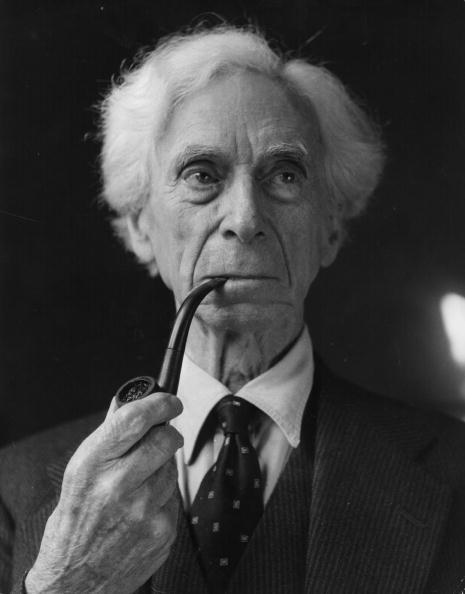
\includegraphics[width=.15\textwidth]{figures/bertrand.png}};
            \node [above = of bertrand] (scene) {Scene};

            \node[sum, right = of bertrand] (sum1) {$+$};
            \node [block, below = of sum1] (atmo-noise) {Atmospheric noise};

            \node [block, right = of sum1] (motion) {Translation, Rotation, Aspect};
            \node [above = of motion] {Motion};

            \node [inner sep=0pt, right = of motion] (motion-output) {};

            \node[inner sep=0pt, below = of motion-output] (bertrand-motion) {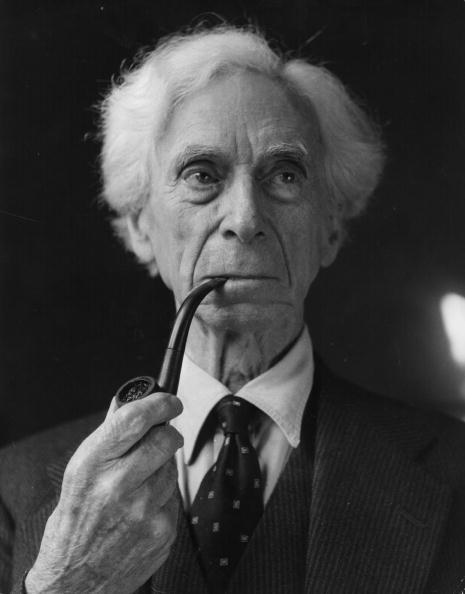
\includegraphics[width=.15\textwidth]{figures/bertrand.png}};
            \node[inner sep=0pt, below = of motion-output, xshift=2mm, yshift=-2mm] {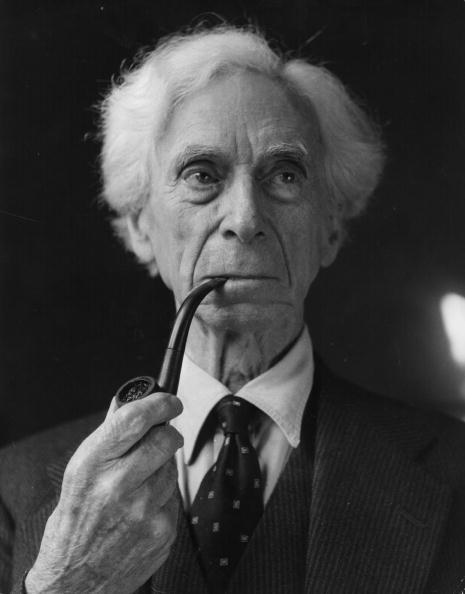
\includegraphics[width=.15\textwidth]{figures/bertrand.png}};
            \node[inner sep=0pt, below = of motion-output, xshift=4mm, yshift=-4mm] {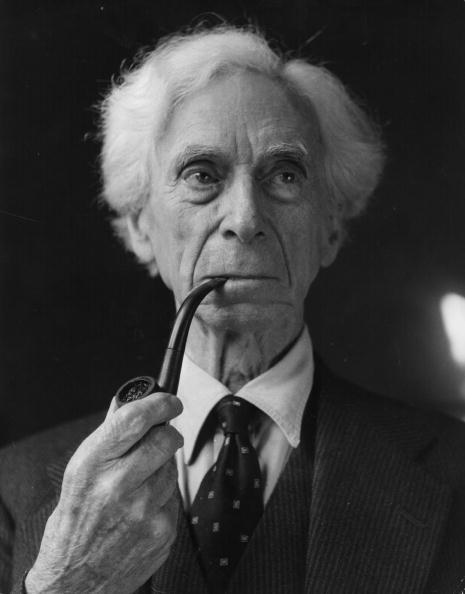
\includegraphics[width=.15\textwidth]{figures/bertrand.png}};
            \node[inner sep=0pt, below = of motion-output, xshift=6mm, yshift=-6mm] {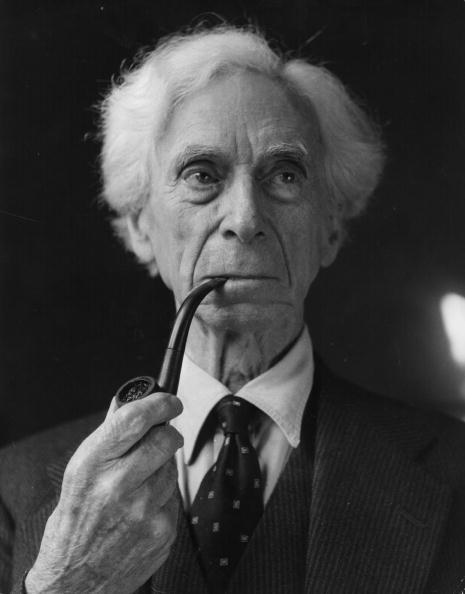
\includegraphics[width=.15\textwidth]{figures/bertrand.png}};

            \node [block, right = of motion-output] (blur) {Optical, Motion};
            \node [above = of blur] {Blur};
            \node [inner sep=0pt, right = of blur] (blur-output) {};

            \node[inner sep=0pt, below = of blur-output] (bertrand-blur) {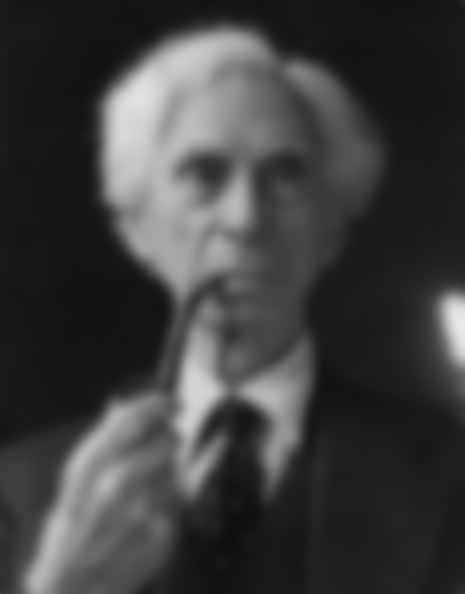
\includegraphics[width=.15\textwidth]{figures/bertrand-blur.png}};
            \node[inner sep=0pt, below = of blur-output, xshift=2mm, yshift=-2mm] {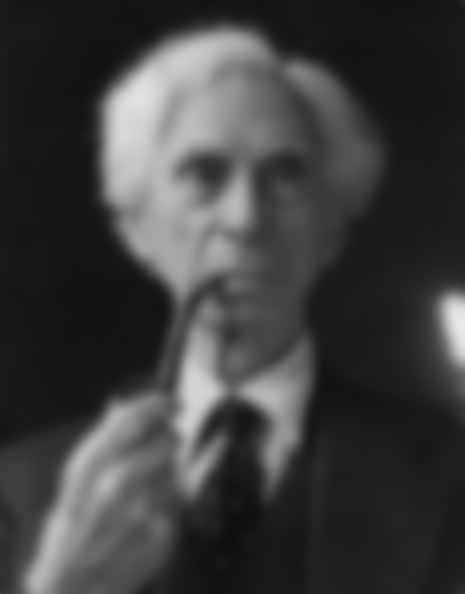
\includegraphics[width=.15\textwidth]{figures/bertrand-blur.png}};
            \node[inner sep=0pt, below = of blur-output, xshift=4mm, yshift=-4mm] {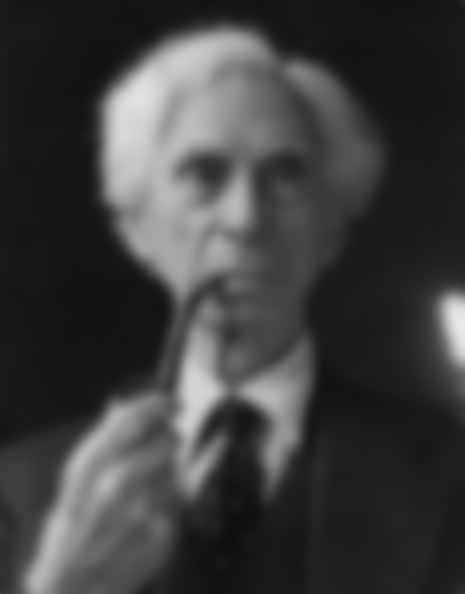
\includegraphics[width=.15\textwidth]{figures/bertrand-blur.png}};
            \node[inner sep=0pt, below = of blur-output, xshift=6mm, yshift=-6mm] {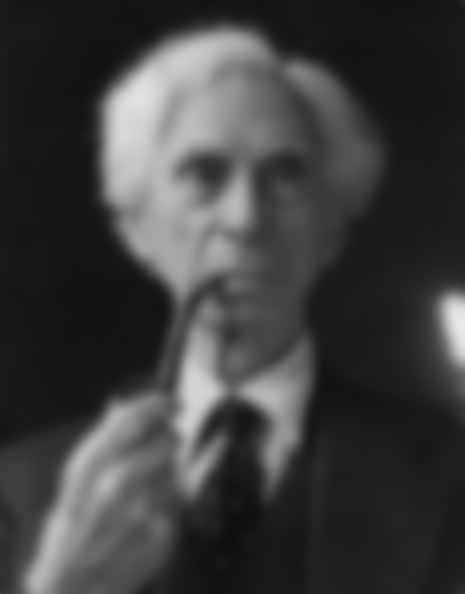
\includegraphics[width=.15\textwidth]{figures/bertrand-blur.png}};

            \node[block, right = of blur-output] (downsample) {Quantization, Pixel-binning};
            \node [above = of downsample] {Down-sampling};

            \node[sum, right = of downsample] (sum2) {$+$};
            \node [block, below = of sum2] (sensor-noise) {Sensor noise};

            \node[inner sep=0pt, right = of sum2] (bertrand-blur-noise) {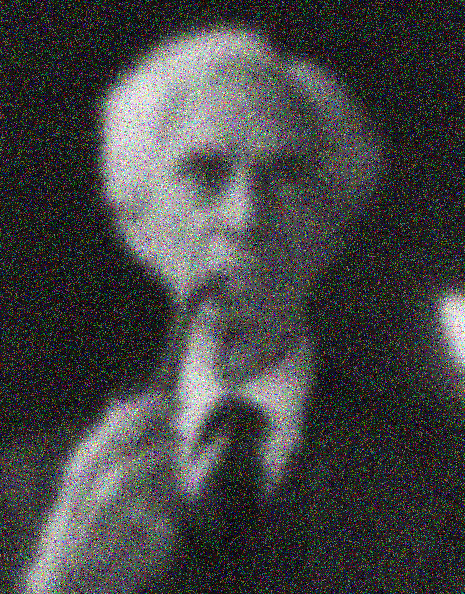
\includegraphics[width=.1\textwidth]{figures/bertrand-blur-noise.png}};
            \node[inner sep=0pt, right = of sum2, xshift=2mm, yshift=-2mm] {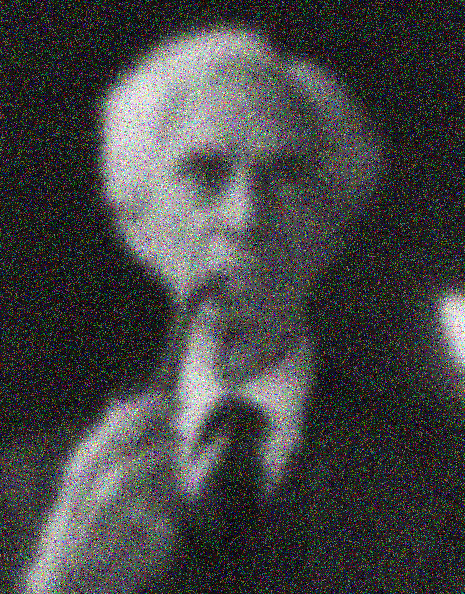
\includegraphics[width=.1\textwidth]{figures/bertrand-blur-noise.png}};
            \node[inner sep=0pt, right = of sum2, xshift=4mm, yshift=-4mm] {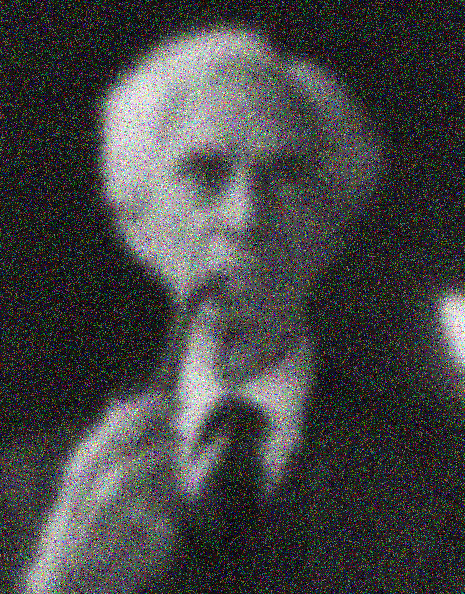
\includegraphics[width=.1\textwidth]{figures/bertrand-blur-noise.png}};
            \node[inner sep=0pt, right = of sum2, xshift=6mm, yshift=-6mm] {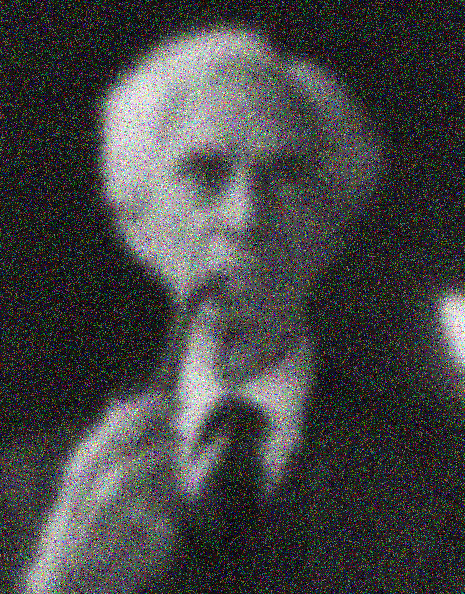
\includegraphics[width=.1\textwidth]{figures/bertrand-blur-noise.png}};
            \node [above = of bertrand-blur-noise, text width=5em] (lr-output) {Low-resolution images};

            \draw[-] (bertrand) edge (sum1);
            \draw[->] (sum1) edge (motion);
            \draw[->] (atmo-noise) edge (sum1);

            \draw[->] (motion) edge (blur);
            \draw[->] (motion-output) edge (bertrand-motion);

            \draw[->] (blur) edge (downsample);
            \draw[->] (blur-output) edge (bertrand-blur);
            \draw[->] (sensor-noise) edge (sum2);
            \draw[-] (downsample) edge (sum2);
            \draw[->] (sum2) edge (bertrand-blur-noise);
        \end{tikzpicture}
    \end{adjustbox}
    \caption{The imaging model illustrating the relationship between a scene and final low-resolution images due to noise, motion, blur, and sampling.}
    \label{fig:bertrand}
\end{figure*}

Let \(Y\) denote an idealized HR image of the scene from some fixed vantage point and assume the imaging system collects \(K\) LR samples \(\Xk\) of \(Y\).
%
Formally the \(\Xk\) are related to \(Y\) by
\begin{equation}
	\Xk = (D \circ H_k \circ A_k) (Y) + \varepsilon_k
	\label{eqn:imagingmodel}
\end{equation}
where for the \(k\)th LR sample, \(A_k\) (of \(K\)) is the operator representing motion, \(H_k\) represents the blur operator, \(D\) represents the down-sampling operator (constant in time since it's typically a digital component of the imaging system), and \(\varepsilon_k\) represents the composite noise (environment and sensor noise).

\subsubsection{Motion}

In the case of MISR, high-resolution images are constructed by exploiting distinct scene data among multiple low-resolution images.
%
Such distinct data are produced by the relative motion of the imaging system and the scene and therefore precise and accurate image \textit{registration}\anote{registration} is paramount.
%
Successful registration is effected by producing a transformation \(f\) that maps pixels at coordinates \((x',y')\) in sample \(\Xkone\) to coordinates \((x,y)\) in sample \(X_j\)
\begin{equation}
	\Xkone(f(x', y')) = X_j(x,y)
	\label{eqn:registration}
\end{equation}
where we use index \(j\) to indicate the possibility of registering all samples relative to a fixed reference image (e.g. \(j=0\) the first sample) or successive/relative registration (i.e.,with \(j=k\)).
%
While image registration is already challenging in the various domains where samples are treated as canonical, such as remote sensing and medical imaging, in SR it is further complicated by the fact that the images to be registered are assumed uncertain.
%
Therefore, in principle, image registration and super-resolution cannot be decoupled, since image registration accuracy would be improved by operating on the estimated HR images;
%
Hardie \etal \cite{Hardie1997} use a Bayesian framework to jointly estimate image registration parameters and the high-resolution image \cite{Hardie1997}.
%
Alternatively one can marginalize over the HR image and estimate the registration parameters using maximum-likelihood estimation (MLE) (see section~\ref{subsubsec:gaussianprocess}).

\subsubsection{Blur}

We now consider the challenges and nuances of estimating blur.
%
In general, the optical transfer function (OTF) characterizes the blur of an imaging system\anote{otf}.
%
We factor the OTF into three components:
\begin{equation}
	H(u, v) \coloneqq H_{\text{diff}}(u,v) H_{\text{abr}}(u,v) H_{\text{int}} (u,v)
\end{equation}
where \(u,v\) are horizontal and vertical spatial frequencies respectively (measured in cycles/mm), \(H_{\text{diff}}\) is blur due to diffraction, \(H_{\text{abr}}\) is blur due to lens aberrations, and \(H_{\text{int}}\) is blur due to imaging sensor shape (obtained by taking the Fourier transform of the shape an individual sensor in the imaging array).
%
Blur due to diffraction in most imaging systems is due to diffraction through a circular aperture \cite{goodman2005introduction}:
\begin{equation*}
	H_{\text{diff}}(u,v) =   \begin{cases}
		\frac{2}{\pi} \left(\frac{1}{\cos(\tau)} - \tau \sqrt{1-\tau^2}\right) & \text{if } \tau < 0 \\
		0                                                                      & \text{otherwise}
	\end{cases}
\end{equation*}
where \(\tau = \rho/\rho_c\), \(\rho=\sqrt{u^2 +v^2}\), \(\rho_c = 1/\lambda N\) is the radial cutoff frequency of the aperture, \(N\) is the f-number\anote{fnumber} of the optics, and \(\lambda\) is the wavelength of light being diffracted.
%
This is in fact the filter that produces the Airy pattern and therefore informs sensor array spacing in order to avoid aliasing.
%
Wavelength independent blurring due to aberrations can be induced by various imperfections in the lenses such as spherical aberration, comatic aberration\anote{coma}, or astigmatism. Furthermore, dispersion\anote{dispersion} blurs particular wavelengths of light. A good model for all of these effects is \cite{10.1117.12.946501}:
\begin{equation*}
	H_{\text{abr}}(u,v) =   \begin{cases}
		1-\left(\frac{25}{65}\right)^2 \left(1-4\left(\tau - \frac{1}{2}\right)\right)^2 & \text{if } \tau < 0 \\
		0                                                                                & \text{otherwise}
	\end{cases}
\end{equation*}
Figure~\ref{fig:mtf} shows an example OTF for an imaging system with a sensor spacing of 0.050 mm and therefore sampling frequency of 20 cycles/mm and \(\rho_c = 83.3~\text{cycles}/\text{mm}\) (\(F=3\) and \(\lambda = 4\mu\text{m}\) i.e.,near infrared).
%
Notice that \(\rho_c\) is much greater than the Nyquist rate (\(\frac{1}{2} \times 20~\text{cycles}/\text{mm} = 10~\text{cycles}/\text{mm}\)) and therefore many frequencies that are within the radial cutoff frequency will be aliased.
%
This in particular can be mitigated by effectively increasing sampling rate using MISR.
%
Notice also that like a typical transfer function the OTF is not flat and therefore attenuates high spatial frequencies.
%
Simply applying gain to the image wouldn't solve the attenuation problems because of aliasing, but likewise this can be resolved after the effective sampling rate is increased using MISR.
\begin{figure}[!htbp]
	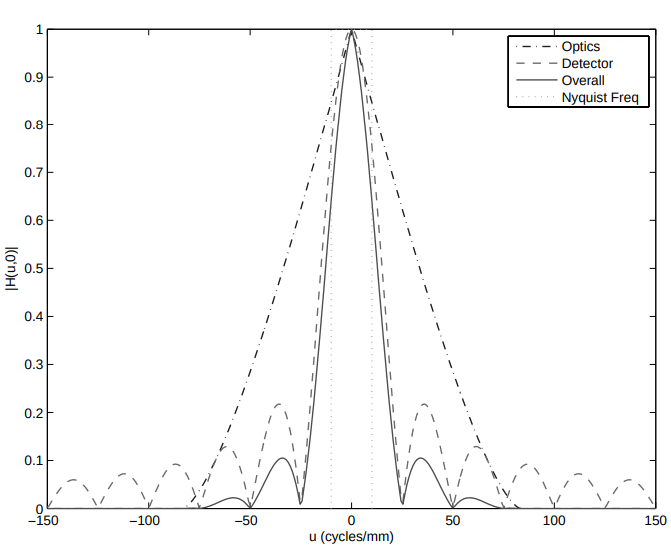
\includegraphics[width=\linewidth,keepaspectratio]{figures/background/mtf.png}
	\caption{OTF magnitude cross-section for \cite{milanfar2017super}.}
	\label{fig:mtf}
\end{figure}

The challenge of super-resolution is to solve the inverse problem of finding \(Y\) from one or several \(\Xk\).
%
In general, since \(A_k, H_k, D_k\) are highly degenerate functions, the corresponding inverse problems are ill-posed without regularization and conditioning.
%
The techniques that have been brought to bear on the problem range from interpolation to statistical estimation to example based learning.
